\chapter{Criação de Cartucho}

O \texttt{MDArte} é composto por uma série de componentes, dentre estes, temos
os cartuchos, um dos mais essenciais e motivo de estudo neste capítulo. Os
cartuchos são responsáveis por prover a habilidade de processar um modelo
utilizando \texttt{Templates}, a fim de gerar o código-fonte. Veremos neste
capítulo que os cartuchos são compostos por vários artefatos, tal como: arquivos
\texttt{XML} de configuração; arquivos para os \texttt{Templates Velocity};
classes \texttt{Java} para as \texttt{Metafacades}; metamodelos de dados
armazenados em um arquivo \texttt{XMI}; etc. E principalmente, como estes
artefatos interagem entre si.

O processo de criação de um cartucho para o \texttt{MDArte} é bastante simples.
Basicamente sendo necessário:
\begin{itemize}
\item Criar, dentro do diretório \texttt{Cartriges} do MDArte, um novo diretório
com o nome que se desja dar ao novo cartucho, tendo, dentro deste, uma estrutura
de diretório padronizada, a fim de armazenar devidamente os artefatos que serão
criados.
\item Criar os arquivos de configuração necessários para a compilação e
funcionamento do cartucho (Ex.: \texttt{cartridge.xml}).
\item Criar os \texttt{Templates Velocity}.
\item Criar o modelo \texttt{UML} que descreve as classes o
cartucho.
\item Recompilar o MDArte.
\end{itemize}

Em alguns casos, veremos que o uso de \texttt{Metafacades} personalizadas será
necessário. A criação de \texttt{Metafacades} será, então, abordada mais à
frente, fazendo com que o processo de criação possuirá etapas adicionais.

\section{Criando a Estrutura de Diretórios}
Primeiramente, crie dentro da pasta \texttt{Cartridges} um diretório com o nome
do novo cartucho. Em seguida, precisamos garantir que a estrutura
de diretório em disco, onde iremos armazenar todos os artefatos para a criação
de um cartucho, esteja correta. Para isso precisamos seguir a seguinte
convenção:

\begin{itemize}
  \item src - Pasta que armazena os artefatos que comporão o cartucho em si.
\end{itemize}

Dentro do diretório \texttt{src}, crie a seguinte estrutura de diretórios:

\begin{itemize}
  \item java - Diretório que armazena os arquivos \texttt{Java} para os
  metafacades do cartucho. Em alguns casos, será necessário a criação do
  subdiretório resources, dentro do diretório \texttt{src}. Este irá conter
  todos os recursos que serão apenas copiados pelo cartucho (Veja logo a seguir
  o elemento \texttt{<resource/>} para maiores explicações).
  \item META-INF - Diretório que armazena arquivos \texttt{XML} que configuram o
  funcionamento do cartucho.
  \item templates - Diretório que armazena os Templates Velocity (Arquivos
  \texttt{VSL}) usados pelo cartucho para gerar os arquivos do sistema final.
  \item uml - Diretório com o metamodelo de dados armazenado em um
	arquivo \texttt{xml.zip}.
\end{itemize}

Dentro do diretório \texttt{META-INF}, crie o diretório \texttt{andromda}, que
armazenará os arquivos de configuração para o \texttt{AndroMDA}.

\section{Criando os arquivos de configuração do cartucho}
Uma vez criada a estrutura de diretórios, o próximo passo será a criação dos
arquivos de configuração do cartucho. 

\subsection{Criando o descritor de configuração do cartucho}
O descritor de configuração nada mais é que um arquivo \texttt{XML}, com o nome
\texttt{cartridge.xml},  e armazenado no subdiretório \texttt{META-INF}, 
seguindo determinadas regras de configuração. (Para maiores informações sobre as
regras a serem seguidas veja o Anexo 1 - Descritor de Configuração do Cartucho
(Schema).) Veremos agora cada elemento do descritor de configuração do cartucho
em detalhes. (Veja o Anexo 2 - Descritor de Configuração do Cartucho (Example).)
O descritor de configuração possuis as seguintes \texttt{tags}:

\begin{enumerate}
	\item <cartridge/> - Elemento raiz para o descritor de configuração do
	cartucho. Possui os seguintes atributos:
	\begin{itemize}

		\item name(*) - Define o nome para o cartucho.

	\end{itemize}

	\item <macrolibrary/> - Este elemento opcional e aninhado com o elemento
	<templateEngine/>, é utilizado para definir uma biblioteca de macros a serem
	utilizados, caso necessário, pelos Templates Velocity. Possui os seguintes
	atributos:

	\begin{itemize}

		\item name(*) - Define o nome do arquivo com a biblioteca de macros (incluindo
		caminho) a serem utilizados pelos os Templates Velocity.

	\end{itemize}

	\item <templateObject/> - Define as classes utilitárias a serem utilizadas pelos
	Templates Velocity. Tais classes poderão ser acessadas por tais Templates a
	partir do nome definido neste elemento. Estas classes precisam definir um
	construtor padrão e precisam estar disponibilizadas para uso pelo cartucho.
	Possui os seguintes atributos:
	
	\begin{itemize}
		\item name(*) - Define o nome pelo qual os Templates Velocity acessarão a
		classe utilitária.
		
		\item className(*) - Nome completo da classe utilitária.
	\end{itemize}

	\item <property/> - Define as propriedades a serem utilizadas pelos Templates
	Velocity. Obs.: As propriedades que não possuírem o atributo default definido
	são obrigatórias. Possui os seguintes atributos:

	\begin{itemize}

		\item reference(*) - Define o nome pelo qual os Templates Velocity acessarão a
		propriedade.

		\item default - Define o valor padrão para a propriedade.

	\end{itemize}

	\item <resource/> -	Define os recursos a serem utilizados pelo cartucho. Os
	recursos, ou melhor, os artefatos, são simplesmente copiados de acordo com o
	valor dos atributos para este elemento <resource/>. Estes não são processados
	por nenhum Template Velocity. Possui os seguintes atributos:
	
	\begin{itemize}

		\item path(*) - Define o caminho, relativo à raiz do cartucho, de um
		recurso a ser copiado para o destino informado pelo atributo outlet.
		Ex.: resources/*.gif
		
		\item outputPattern(*) - Define o local dentro do caminho de destino informado
		pelo atributo outlet, onde será copiado cada arquivo de recurso. Ex.:
		pages/images/\{0\}, onde \{0\} é o nome do recurso no momento processado.
		
		\item outlet(*) - Define o caminho lógico de destino onde o recurso será copiado.
		
		\item overwrite(*) - Define se um recurso deverá ser sobrescrito, caso este já exista no caminho de destino informado pelo atributo outlet.
		
		\item required - Define se este recurso será obrigatório ou não para a aplicação
		que for utilizar tal cartucho.
	
	\end{itemize}

	\item <template/> - Define os Templates Velocity a serem utilizados para a
	geração do código-fonte. Possui os seguintes atributos:
	
	\begin{itemize}

		\item path(*) - Define o caminho, relativo à raiz do cartucho, de um Template
		Velocity a ser utilizado.
		
		\item outputPattern(*) - Define o local dentro do caminho de destino informado
		pelo atributo outlet, onde o arquivo, contendo o código-fonte produzido pelo
		Template Velocity, será gerado. Ex.: \{0\}/\{1\}Bean.java, onde \{0\} é o nome
		do pacote definido no modelo, e \{1\} é o nome para o elemento de modelo
		processado.
		Obs: Uma variável do Template Velocity pode ser informada (Ex.:
		\textdollar{}generatedName )  esde que esta seja configurada no Template
		correspondente.
		
		\item outlet(*) - Define o caminho lógico de destino onde o arquivo, contendo o
		código-fonte produzido pelo Template Velocity, será gerado.
		
		\item overwrite(*) - Define se o arquivo, contendo o código-fonte produzido pelo
		Template Velocity, deverá ser sobrescrito, caso este já exista no caminho de
		destino informado pelo atributo outlet.
		
		\item generateEmptyFiles - Define se os arquivos deverão ser criados mesmo que
		nenhum resultado seja gerado pelo Template Velocity. Geralmente utilizado para
		gerar o arquivo baseado em alguma informação do modelo.
		
		\item outputToSingleFile - Define caso seja necessário gerar um único arquivo
		para todos os elementos de modelo agregados. Por exemplo: Bastante útil para a
		geração de scripts SQL.
		
		\item outputOnEmptyElements - Este atributo apenas terá sentido caso o atributo
		outputToSingleFile esteja com o valor true. Define se mesmo que não haja
		elementos de modelo agregados, o arquivo deverá ser gerado.
		
		\item required - Define se este recurso será obrigatório ou não para a aplicação
		que for utilizar tal cartucho.

	\end{itemize}

	\item <modelElements/> - Este elemento aninhado com o elemento <template/>, é
	utilizado para informar ao Template Velocity quais os elementos de modelo
	deverão ser processados. Possui os seguintes atributos:

	\begin{itemize}
		\item variable - Define a variável (Ex.: \textdollar{}entity) que estará
		disponibilizada para utilização no Template Velocity.
	\end{itemize}

	\item <modelElement/> - Este elemento aninhado com o elemento <modelElements/>,
	é utilizado para informar ao Template Velocity qual elemento de modelo deverá
	ser processado. Possui os seguintes atributos:

	\begin{itemize}
		\item stereotype - Define o nome do esteriótipo que o elemento de
		modelo precisa ter para que este esteja disponível para uso no Template
		Velocity. Este campo não é obrigatório, pois o elemento aninhado <type/> pode
		ser utilizado, ao invés deste atributo.
		\item variable - Define a variável que estará disponibilizada para utilização
		no Template Velocity. O uso deste atributo apenas terá sentido caso o atributo
		outputToSingleFile esteja com o valor true, atentando ao fato de que sendo
		suficiente, na maioria dos casos, apenas o atributo variable para o elemento
		<modelElements/>.
		Em combinação com o atributo outputToSingleFile, este atributo permite agrupar
		elementos de modelo e torná-los disponíveis para os Templates Velocity.
	\end{itemize}

\begin{figure}[H]
	\centering
	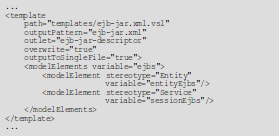
\includegraphics[width=380pt,height=180pt]{files/imgs/apendice-cartucho-novo-00001.png}
	\caption{Exemplo de uso da propriedade modelElement.}
	\label{exemplo_model_element}
\end{figure}

No exemplo acima, todos os elementos de modelo com os estereótipos
\texttt{<<Entity>>} e \texttt{<<Service>>} estarão disponíveis para os Templates
Velocity sob as variáveis \textdollar{}entityEjbs e \textdollar{}sessionEjbs,
respectivamente. Mas também haverá uma variável \textdollar{}ejbs que estará
disponível para os Templates Velocity, contendo tanto os elementos de modelo com
o esteriótipo \texttt{<<Entity>>}, quanto os elementos de modelo com o
esteriótipo \texttt{<<Service>>}.

\item <type/> - Este elemento opcional e aninhado com o elemento
<modelElement/>, é utilizado para informar ao Template Velocity qual elemento de
modelo deverá ser processado. Os elementos de modelo a serem processados serão
aqueles que estiverem associados à Metafacade definida pelo atributo name. Não é
necessário utilizar tal elemento caso o atributo stereotype do elemento
<modelElement/> esteja definido. Possui os seguintes atributos:

\begin{itemize}
  \item name(*) - O nome completo da classe para o Metafacade.
\end{itemize}

\item <property/> - Este elemento opcional e aninhado com o elemento <type/>, é
utilizado para informar ao Template Velocity qual elemento de modelo deverá ser
processado. Os elementos de modelo a serem processados serão aqueles que
estiverem associados à Metafacade definida pelo atributo name do elemento
<type/> acima, e caso esta Metafacade associada possua uma das propriedades
definidas por este elemento. Posui os seguintes atributos:

\begin{itemize}
  \item name(*) - O nome da propriedade para o Metafacade.
  \item value - O valor da propriedade para o Metafacade.
\end{itemize}

É importante atentar para o fato de que não é necessário especificar uma valor
para uma propriedade. Assim, caso o atributo value não seja especificado, a
propriedade precisa apenas ser válida: seja não-nula, possua um ou mais
elementos caso seja uma coleção ou seja verdadeira caso seja um tipo boolean.

Obs.: Atributos com o símbolo (*) são obrigatórios.

\subsection{Criando o arquivo de configuração do perfil do cartucho}
Crie no diretório \texttt{META-INF > andromda}, o arquivo \texttt{profile.xml}.
Este arquivo \texttt{XML} é reponsável por registrar os estereótipos e valores
etiquetados que serão usados pelo cartucho na interpretação do modelo. O arquivo
possui as seguintes \texttt{tags}:

\begin{itemize}
  \item <profile> - Raiz da configuração, deve englobar todas as demais tags.
  \item <documentation> - Descrição do que é o cartucho, seu intuito e demais
  informações que se julgue necessárias.
  \item <elements> - Tag que engloba a lista de elementos (estereótipos e
  valores etiquetados) a serem definidos.
  \item <elementGroup> - Devendo ser colocada dentro de <elements>, esta tag
  nos permite criar grupos de elementos definidos dentro de si e a usaremos para
  separar os elementos de acordo com o seu tipo. Esta tag possui uma propriedade
  \texttt{`name`}, usada para definir o nome do grupo criado (Ex.: Stereotypes).
  \item <element> - Devendo ser colocada dentro de um <elementGroup>, esta tag
  define um elemento a ser usado no modelo. Tem suas propriedades definidas com
  outras tags dentro de si. Cada elemento deve conter dentro de si as seguintes
  tags:
  \begin{enumerate}
    \item <documentation> - Descrição sobre o estereótipo sendo registrado.
    \item <value> - Valor, em texto, associado àquele estereótipo.
    \item <appliedOnElement> - Tipo de elemento \texttt{UML} ao qual tal
    estereótipo deve ser aplicado. Se queremos que ele só seja aplicado a
    classes, por exemplo, definiremos 
    `\texttt{<apliedOnElement>class<apliedOnElement/>}`.
  \end{enumerate}
\end{itemize}

\end{enumerate}

\subsection{Criando arquivo de configuração dos metafacades do cartucho}
Vamos falar agora sobre o arquivo de configuração dos metafacades criado
especficamente para o cartucho criado. Veremos agora as tags que compõe esse
arquivo e posteriormente, quando criarmos os metafacades personalizados,
criaremos a sua configuração de acordo com o padrão visto a seguir. Obs: este
arquivo só é necessário caso haja metafacades personalizados, caso contrário,
não precisa ser criado.

O Arquivo possui a seguinte estrutura de tags:

\begin{itemize}
  \item <metafacades/> - É a raiz do arquivo, englobando todo o resto da 
  configuração. 
  \item <property/> - A tag raiz (<metafacades/>) pode ter tantos <property/>
  quanto necessário, inclusive nenhum. Tais tags registram propriedades
  de namespace que podem definir referências a uma variável ou valores default,
  sendo estes definidos em um arquivo andromda.xml. Esta tag possui os seguintes
  atributos:
  \begin{enumerate}
    \item reference - Atributo obrigatório. Especifica a propriedade
    externamente configurada a qual se está fazendo referência.
    \item default - Atributo não obrigatório. Fornece um valor default para o
    atributo, para o caso de tal propriedade não estar configurada externamente.
  \end{enumerate}
  
  \item <default/> - Esta tag é opcional, no entanto, dentro de <metafacades/>
  pode haver no máximo uma única tag <default/>. Esta define um metafacade a ser
  usado para mapear um elemento para o qual não seja encontrado nenhum outro
  metafacade que o mapeie. Possui o atributo \texttt{`class`} que define o nome
  da classe do metafacade usado para mapear os elementos. 
  \item <metafacade/> - Permite configurar um mapeamento de um elemento do
  modelo para uma classe de metafacade. Deve ser criada dentro da tag
  <metafacades/>. Possui as seguintes propriedades:
  \begin{enumerate}
    \item class - Define o nome
    da classe do metafacade usado para mapear os elementos do modelo.
    \item contextRoot - Atributo booleano não obrigatório que indica se
    um dado metafacade serve de contextRoot (`raiz de contexto`) para
    outro metafacade, ou seja, se um outro metafacade será instanciado
    no contexto do metafacade que se está mapeando. O mapeamento abaixo, por
    exemplo, indica que o metafacade construído a partir de
    WebServiceLogicImpl será contextRoot, já que teremos
    WebServiceOperationLogicImpl usando o metafacade anterior como base para a
    construção de seu contexto.
    
    \begin{lstlisting}[language=xml]
	...
	<metafacade
		class="org.andromda.cartridges.webservice.metafacades.WebServiceLogicImpl"
		contextRoot="true"> 
		<mapping class="org.omg.uml.foundation.core.UmlClass$Impl">
			<stereotype>WEBSERVICE</stereotype> 
		</mapping> 
	...
	</metafacade>
	...
	<metafacade
		class="org.andromda.cartridges.webservice.metafacades.WebServiceOperationLogicImpl"
		contextRoot="true">
		<mapping class="org.omg.uml.foundation.core.Operation$Impl">
			<context>org.andromda.cartridges.webservice.metafacades.WebService</context> 
		</mapping> 
	...
	</metafacade>
	...
	\end{lstlisting}
  \end{enumerate}
  
  \item <property/> - Tag opcional, dentro da tag <metafacade/>, podendo cada
  metafacade ter tantas referências a propriedades quanto necessário.
  Similarmente às propriedades de namespace aneteriormente descritas, podemos
  definir referências a propriedades externamente configuradas no escopo de um
  único metafacade. Isto nos permite configurar um valor específico de
  propriedade para um metafacade, sem precisar alterar o valor dessa propriedade
  no escopo do cartucho.
  \item <mapping/> - Cada metafacade deve ter uma única tag <mapping/>
  dentro de si. A tag <mapping/> contém as informações que deixam claro pro
  MDArte de que forma um elemento do metamodelo deve ser mapeado para um
  metafacade específico. O mapping pode ser feito a partir da combinação dos
  seguintes atributos, a serem detalhados posteriormente:

  \begin{enumerate}
    \item stereotype 
    \item context
    \item property
  \end{enumerate}
  
  \item <stereotype/> - Tag opcional. Cada <mapping/> pode ter uma ou mais tags
  <stereotype/> dentro de si. Define que a marcação de determinado estereótipo
  seja usada como forma de definir qual metafacade será usado para mapear um
  elemento do metamodelo.
  
  \item <context/> - Tag opcional. Cada <mapping/> pode ter um único
  <context/>. Cada elemento do metamodelo pode ser mapeado por um único
  contexto. Um contexto é o nome da interface associada a uma classe de
  metafacade, devendo ser o contexto a partir do qual o metafacade é
  construído.
  
  \item <property/> - Tag opcional. Cada <mapping/> pode ter uma ou mais
  <property/>. Propriedades podem ser definidas com um valor específico ou sem
  um valor definido. Quando mapeada sem um valor definido, a propriedade
  precisará ser considerada válida para que um elemento seja a associado ao
  <mapping/> que a engloba. Uma propriedade é considerada válida nos seguintes
  casos:
  
  \begin{itemize}
    \item A propriedade tem valor não nulo.
    \item Se um atributo é uma Collection e esta não está vazia.
    \item Se um atributo booleano não é falso.
  \end{itemize}
  
\end{itemize}

\subsection{Criando o arquivo de configuração do Namespace do cartucho}
Crie no diretório \texttt{META-INF > andromda}, o arquivo
\texttt{namespace.xml}. Este arquivo \texttt{XML} é responsável por registrar as
propriedades e variáveis globais que estarão disponíveis para os templates do
cartucho, bem como registrar os componentes do mesmo. O arquivo é composto das
seguintes tags:

	\begin{itemize}
	  \item <namespace> - Raiz da configuração, devendo englobar todas as tags
	  seguintes. Possui o atributo \texttt{name}, que define o nome do namespace
	  que se está definindo.
	  \item <components> - Define um conjunto de componentes de configuração a
	  serem registrados como parte do cartucho. Deve englobar as tags <component>
	  \item <component> - Registra um componente de configuração do cartucho.
	  Usaremos esta tag para registr os outros arquivos de configuração
	  anteriormente criados. Possui o atributo \texttt{name}, que define o nome do
	  componente, devendo ser preenchido com o mesmo nome do arquivo, sem a
	  extensão, ou seja, para o arquivo \texttt{cartridge.xml}, definiremos
	  \texttt{`name`=`catridge`}.
	  \item <path> - Define o caminho onde está localizado um componente de
	  configuração, devendo, portanto, ser definida dentro da tag <component>. É
	  importante notar que o caminho é definido considerando novo-cartuco/src como
	  a raiz do projeto, não devendo este caminho ser especificado. Para definir o
	  path para o arquivo \texttt{cartridge.xml}, que criamos no caminho,
	  novo-cartuco/src/META-INF/andromda, basta definir \texttt{<path>
	  META-INF/andromda/profile.xml}.
	  \item <properties> - Define um conjunto de propriedades do cartucho.
	  \item <propertyGroup>	- Define um grupo de propriedades, agrupadas
	  logicamente de acordo com o seu intuito. Deve conter obrigatoriamente um
	  atributo \texttt{name}, que define o nome do grupo sendo definido. Dentro
	  desta tag, serão definidas as propriedades referentes a tal grupo e,
	  opcionalmente, uma tag <documentation>, com alguma descrição sobre tal grupo 
	  de propriedades. Deve ser definida dentro da tag <properties>.
	  \item <property> - Define uma propriedade do cartucho. Cada propriedade
	  funciona como uma variável `global` do cartucho, acessível a todos os seus
	  templates. Uma propriedade deve ter, obrigatoriamente, o atributo `name`, que
	  define o nome daquela propriedade, e, opcionalmente, o atributo booleano
	  `required`, que determina se tal propriedade precisa ter um valor definido
	  para si no arquivo \texttt{XML} de configuração do \texttt{AndroMDA}
	  (\texttt{andromda.xml}). Caso `required` seja definido como \texttt{true}, o
	  AndroMDA emitirá uma warning caso a tal propriedade não tenha um valor
	  definido para si. Além disso, pode-se configurar propriedades adicionais em
	  uma <property>, definindo dentro dela as seguintes tags (nenhuma delas
	  obrigatória):
	  \begin{enumerate}
	    \item <default> - Valor default para tal propriedade.
	    \item <documentation> - Descrição da propriedade sendo definida.
	  \end{enumerate}
	\end{itemize}

Obs.: Você pode notar que dependendo da forma como os mapeamentos para os
metafacades são registrados e definidos pode acontecer de um determinado
elemento ter mais de um mapeamento compatível. É importante ter em mente que,
nesses casos, a ordem dos mappings no arquivo interfere diretamente no
mapeamento dos elementos, uma vez que o MDArte aproveitará o primeiro mapeamento
válido declarado no arquivo. Isso quer dizer que no caso de querer declarar dois
tipos de mapeamento para um mesmo estereótipo, por exemplo, um mais geral e
outro mais detalhado, o ideal seria declarar o mais detalhado primeiro e depois
o menos detalhado. Nesse caso, caso um elemento não fosse mapeado pelo
mapeamento mais restrito, ele ainda poderia ser casado com o mapeamento mais
amplo.

\section{Criando os arquivos .properties}
Criaremos os seguintes arquivos \texttt{.properties} que serão usados pelo
\texttt{Maven} durante a geração e compilação dos cartuchos do MDArte. Crie os
arquivos \texttt{mda.properties} e \texttt{project.properties} dentro da pasta
raiz do cartucho.

Crie o arquivo \texttt{mda.properties} com o seguinte conteúdo:

\lstinputlisting[language=bash, frame=single]{files/properties/mda.properties}

Crie com o arquivo \texttt{project.properties} com o seguinte conteúdo:

\lstinputlisting[language=bash, frame=single]{files/properties/project.properties}

As propriedades \texttt{metafacade.model.file} e
\texttt{maven.andromda.model.uri} definem, respectivamente, o caminho para o
arquivo \texttt{xml.zip} que contém o modelo UML dos metafacades do cartucho e o
caminho para o arquivo \texttt{XML} do modelo, que encontra-se empacotado no
\texttt{xml.zip}.

\section{Criando os arquivos de dependências de compilação do cartucho
(project.xml e pom.xml)}
O arquivo \texttt{pom.xml} é o reponsável por descrever o projeto sendo
automatizado para o \texttt{Maven}, contendo desde informações sobre os
desenvolvedores e a \texttt{url} onde o projeto reside, até arquivos de
configuração e algumas dependências de projeto. Veja abaixo um exemplo de
\texttt{pom.xml}, para ser usado no cartucho que criamos:

\lstinputlisting[language=xml, frame=single]{files/xml/novo-cartucho-project.xml}

Não se esqueça de mudar as propriedades \texttt{<name>} e \texttt{<artifactId>}
para refletir os valores desejados para o projeto em questão. Mais informações
sobre o funcionamento do arquivo \texttt{pom.xml} neste
\href{http://maven.apache.org/pom.html}{link}\footnote{\href{http://maven.apache.org/pom.html}{http://maven.apache.org/pom.html}}.

O arquivo \texttt{project.xml}, no MDArte, é o reponsável por registrar
as dependências e outras características específicas do projeto sendo
desenvolvido. Vale lembrar que o MDArte permite a criação de múltiplos arquivos
\texttt{project.xml}, a fim de que cada unidade menor do projeto possa definir
de forma local as dependências que só dizem respeito a si. Veja abaixo um
exemplo de \texttt{project.xml}, para ser usado no cartucho que criamos:

\lstinputlisting[language=xml,
frame=single]{files/xml/novo-cartucho-project.xml}

Não se esqueça de mudar as propriedades \texttt{<name>}, \texttt{<artifactId>} e
quaisquer outras que sejam necessárias para refletir os valores desejados
para o projeto em questão. Mais informações sobre o funcionamento do arquivo
\texttt{pom.xml} neste
\href{http://maven.apache.org/pom.html}{link}\footnote{\href{http://maven.apache.org/pom.html}{http://maven.apache.org/pom.html}}.

\subsection{Criando arquivo de ações do maven (maven.xml)}
Este arquivo é responsável por definir quais tipos de ações o \texttt{Maven}
executará para o cartucho. Abaixo temos um exemplo de configuração simples,
porém suficiente para a maioria dos cartuchos.

\lstinputlisting[language=xml,
frame=single]{files/xml/novo-cartucho-maven.xml}

\section{Criando os Templates Velocity}
O processo de criação dos Templates Velocity é bastante simples. Basicamente
precisamos criar para cada elemento <template/> definido no descritor de
configuração do cartucho (andromda-cartridge.xml), um arquivo VSL
correspondente. (Para maiores informações sobre Templates Velocity veja o Anexo
3 - Templates Velocity User Guide.) Veja abaixo um exemplo de arquivo VSL. Este
Template Velocity é utilizado para gerar um arquivo de propriedades para o
Struts Framework, definindo os nomes dos campos de formulários, assim como os
títulos das páginas a partir dos elementos de modelo.

\begin{figure}[H]
	\centering
	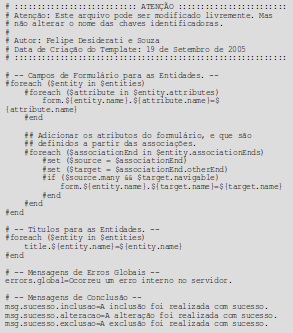
\includegraphics[width=280pt,height=260pt]{files/imgs/apendice-cartucho-novo-00005.png}
	\caption{Exemplo de Arquivo Velocity.}
	\label{exemplo_velocity}
\end{figure}